\section*{Solutions}


\begin{figure}[H]
\centering

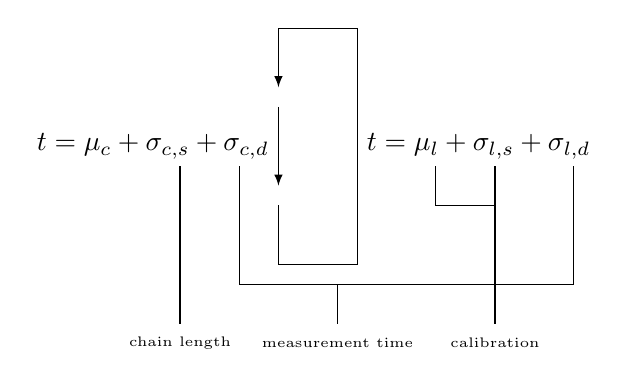
\begin{tikzpicture}

\draw [>=latex,->]
(0,1.25) |-
(1,0.5) --
(1,3.5) -|
(0,2.75);

\draw [>=latex,->]
(0,2.5) --
(0,1.5);

\node [anchor=west] at (1,2) {$t=\mu_l+\sigma_{l,s}+\sigma_{l,d}$};
\node [anchor=east] at (0,2) {$t=\mu_c+\sigma_{c,s}+\sigma_{c,d}$};

% measurement time
\draw [](-0.5,1.75) -- (-0.5,0.25) -|  (0.75,-0.25);
\draw (0.75,0.25) -| (3.75,1.75);
\node at (0.75,-0.5) {\tiny{measurement time}};

% callibration
\draw (2.75,-0.25) -- (2.75,1.75);
\draw (2,1.75) |- (2.75,1.25);
\node at (2.75,-0.5) {\tiny{calibration}};

% chain length
\draw (-1.25,-0.25) -- (-1.25,1.75);

\node at (-1.25,-0.5) {\tiny{chain length}};
\end{tikzpicture}

\caption{math}
\label{tkz:math}
\end{figure}


\begin{align}
\sigma_{tot} = \sqrt{\frac{\sigma_{c,s}^2}{\text{components}}+\frac{\sigma_{c,d}^2+\sigma_{l,d}^2}{\text{counts}}}
\end{align}

\begin{align}
LSB = \frac{t_{period}^2}{t_{measurement}}
\end{align}